%!TEX program = xelatex
% Note: this template must be compiled with XeLaTeX rather than PDFLaTeX
% due to the custom fonts used. The line above should ensure this happens
% automatically, but if it doesn't, your LaTeX editor should have a simple toggle
% to switch to using XeLaTeX.

\documentclass[
  aspectratio=169, % Uncomment to use an aspect ratio of 16:9 (160 mm by 90 mm)
  %aspectratio=43, % Uncomment to use an aspect ratio of 4:3 (128mm by 96mm)
  t, % Top align all slide content by default
  onlytextwidth, % Typeset content in columns at text width
  10pt, % Default font size, use 10pt for the 16:9 aspect ratio and 8pt for the 4:3 aspect ratio
]{beamer}

\usepackage{../../ImperialTheme/beamer/beamerthemeImperial} % Use the Imperial theme

\def\imagefolder{../../ImperialTheme/beamer/Images}
\def\Rey{\text{Re}}
\title{Blowing Suction in flat plate} % Presentation title to appear on the title slide and left footers

\subtitle{} % Presentation subtitle to appear on the title slide

\author{Víctor Ballester} % Author name(s) to appear on the title slide

\date{\today} % Presentation date to appear on the title slide and right footers

\begin{document}

\begingroup
\setbeamercolor{background canvas}{bg=ICLBlue} % Slide background color
\setbeamercolor{title page title}{fg=white} % Title text color
\setbeamercolor{title page subtitle}{fg=white} % Subtitle text color
\setbeamercolor{author}{fg=white} % Author(s) text color
\setbeamercolor{date}{fg=white} % Date text color
\setbeamertemplate{title page}[logo]{\imagefolder/ICL_Logo_White.pdf} % Imperial logo color, use 'ICL_Logo_White.pdf' for white and 'ICL_Logo_Blue.pdf' for blue
\frame[plain, s]{\titlepage} % Output the title page with no footer ('plain') and vertically distributed text ('s')
\endgroup

\begin{frame}
	\frametitle{Blowing and suction}
	\begin{itemize}
		\item I modify the BC of $v$ on the wall with:
		      $$
			      v(x,t)= A \sin\theta(1-\cos\theta)\sin(\omega t) {\bf{1}}_{x\in (x_0, x_0 + \ell)}
		      $$
		      where $A=0.003$, $x_0=0$ (for the flat plate!), $\ell = 2\pi/\alpha_r$, $\omega=\omega_r$ and $\theta = \alpha_r (x-x_0)$. The pair $(\alpha_r, \omega_r)$ is taken from Orr-Sommerfeld eq. Probably I will increase a little bit $\omega$ because $\omega_r$ is very small.
		\item I found the function $\sin\theta (1-\cos\theta)$ in a paper. I assume they use it to make a $\mathcal{C}^2$ contact as well as keep the integral of the curve big, in order to ``maximize" the forcing.
		\item Orr-Sommerfeld analysis for $w=15$:
	\end{itemize}

	\begin{columns}[T] % [T] ensures correct vertical alignment
		\begin{column}{0.32\linewidth} % Left column
			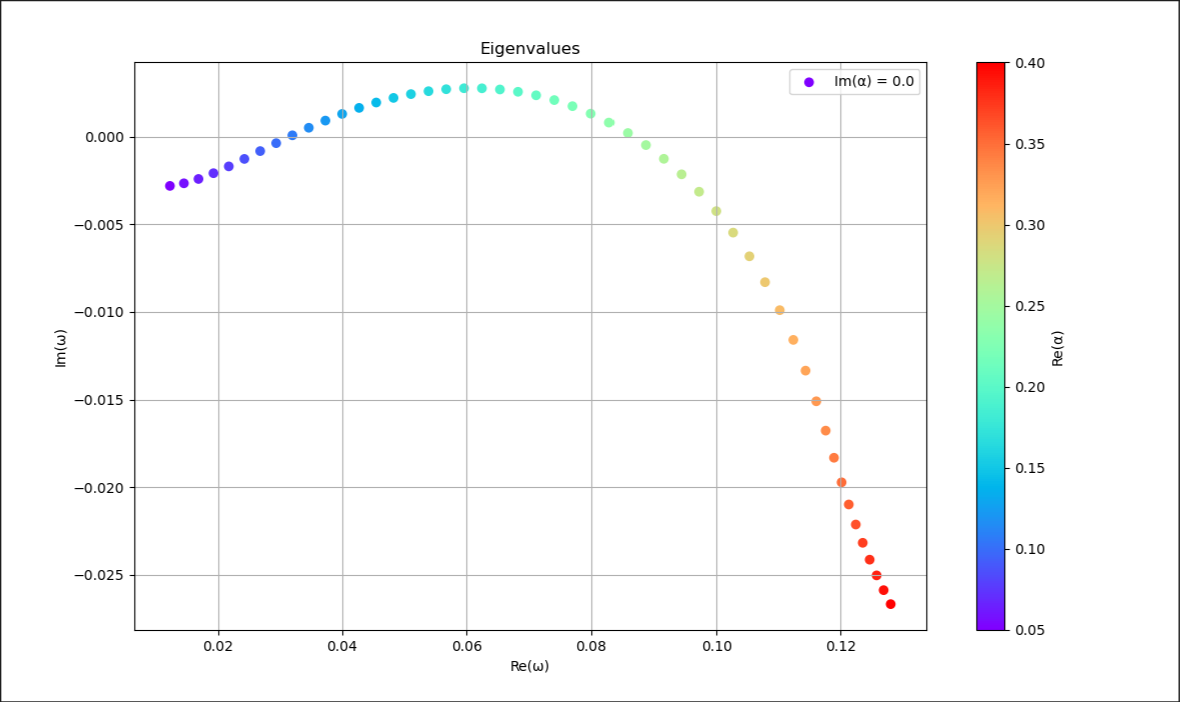
\includegraphics[width=\linewidth]{Images/osX15.png}
			$x=15\delta^*$ (downstream edge)
		\end{column}
		\begin{column}{0.32\linewidth} % Left column
			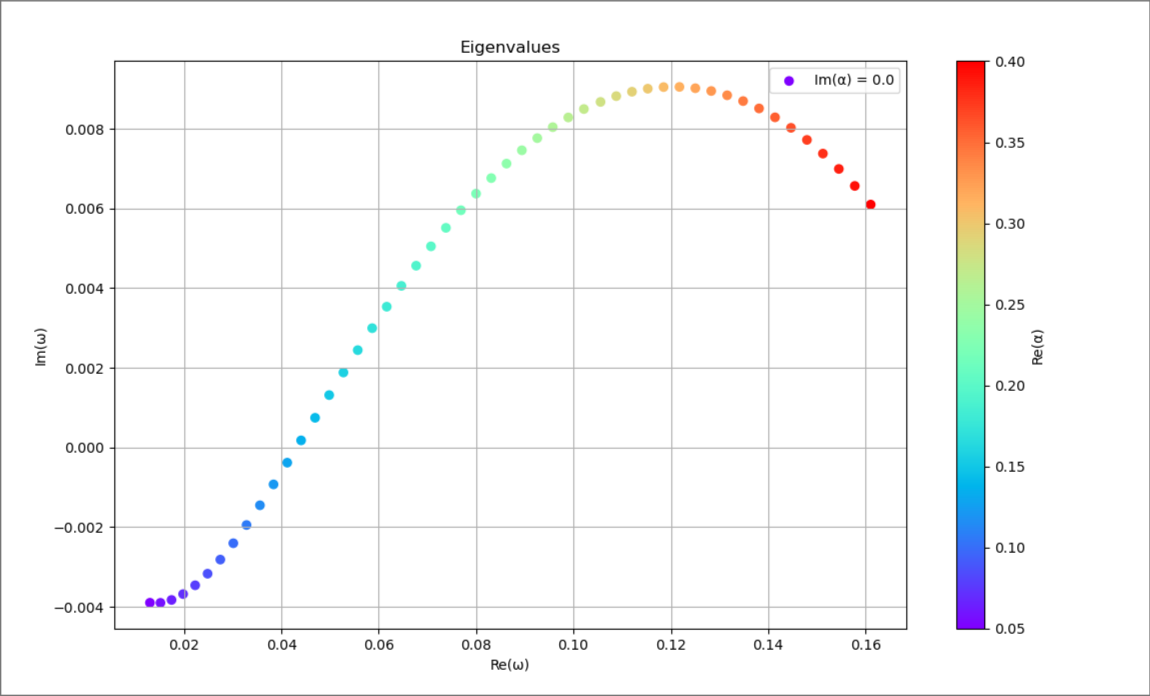
\includegraphics[width=\linewidth]{Images/osX300.png}
			$x=300\delta^*$ (downstream edge)
		\end{column}
		\begin{column}{0.32\linewidth} % Left column
			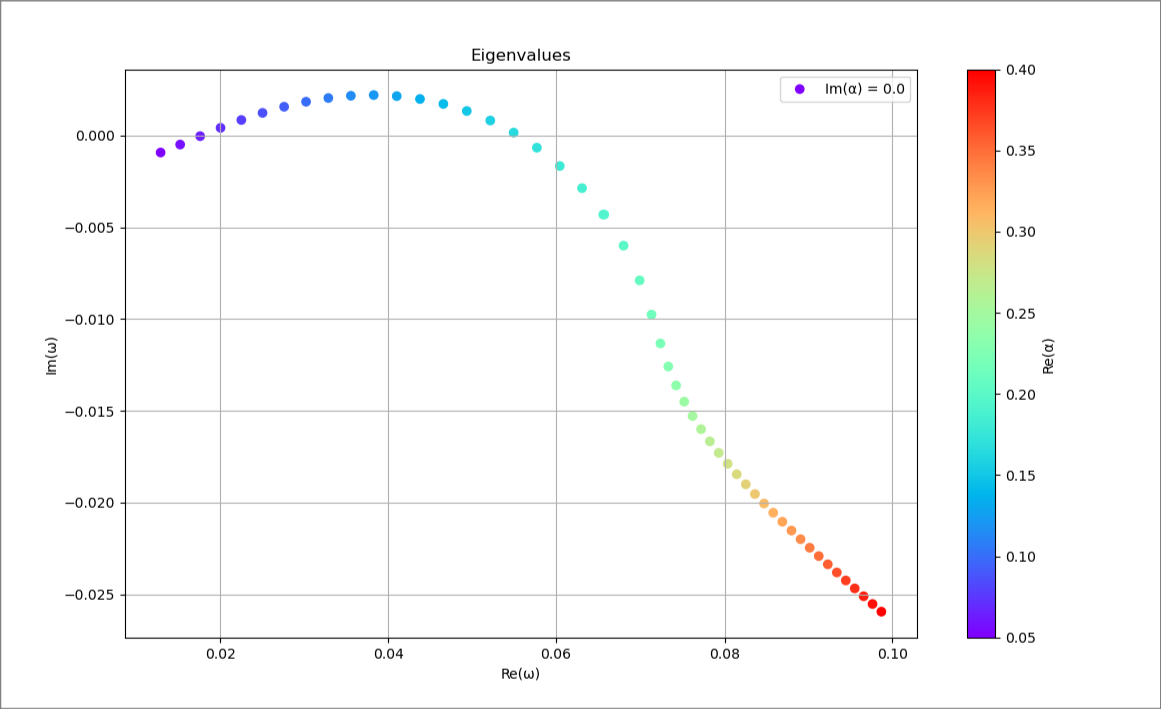
\includegraphics[width=\linewidth]{Images/osX900.png}
			$x=900\delta^*$ (downstream edge)
		\end{column}
	\end{columns}
\end{frame}
\begin{frame}
	\frametitle{Flat DNS TS amplitudes}
	\begin{itemize}
		\item Evolution of different points in the domain of the $u$ (left) and $v$ (right) fields (linear solver with blowing and suction).
	\end{itemize}
	\centering
	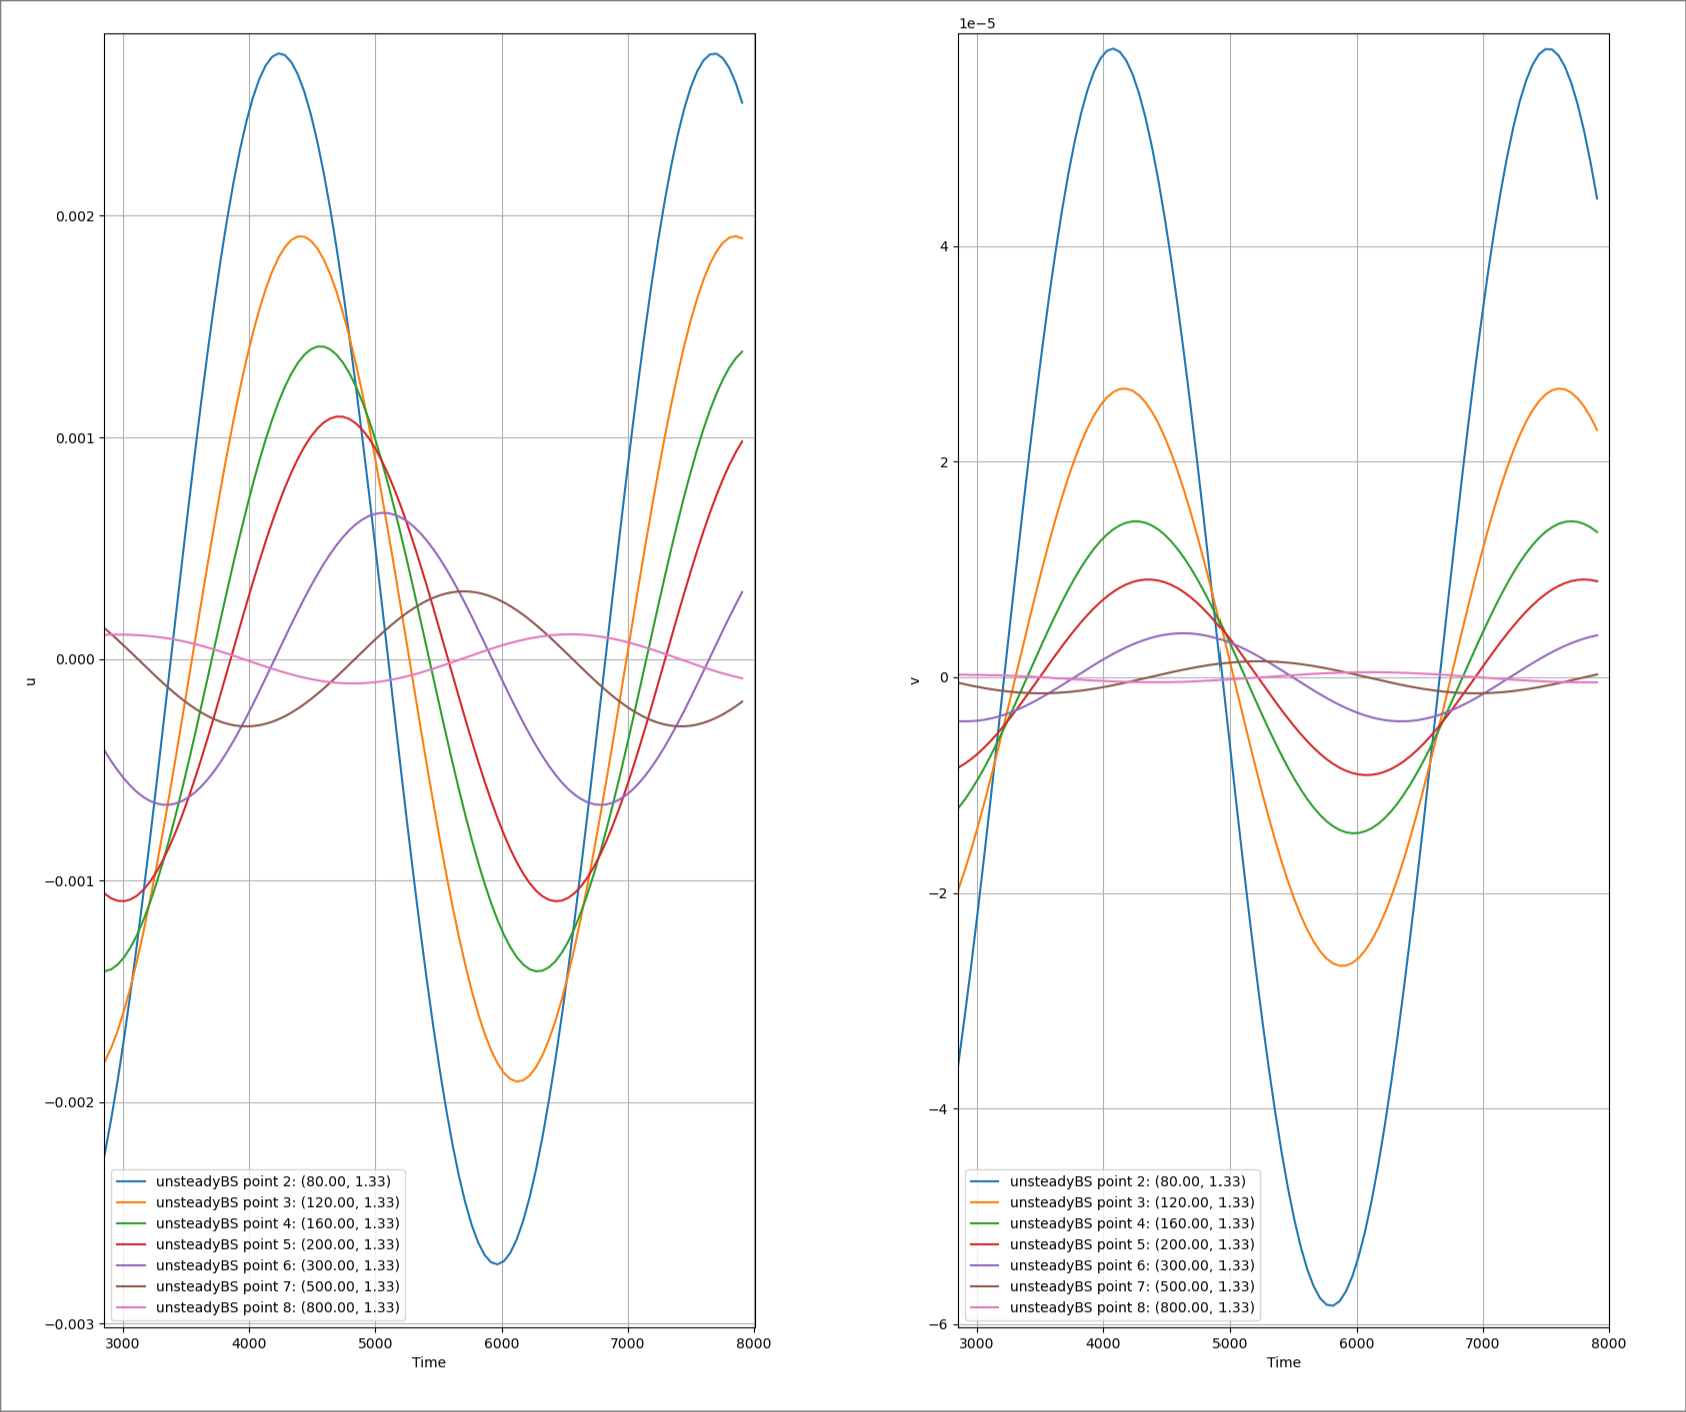
\includegraphics[width=0.5\linewidth]{Images/TS_amplitudeDNS_flat.png}
\end{frame}
\begin{frame}
	\frametitle{General comments}
	\begin{itemize}
		\item Should I increase the upstream region for blowing and suction in the gap version?
	\end{itemize}
	\centering
	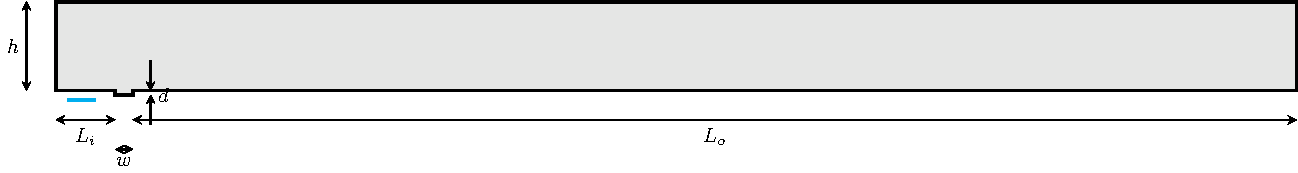
\includegraphics[width=1\textwidth]{../../Images/domainBS.pdf}
	\begin{itemize}
		\item I was not able to make the Coupled direct solver work, but I haven't tried too much.
		\item I have all the ingredients to compute the $n(x)$ curves. I am in the postprocessing part now.
		      % \item To compute 
		      $$
			      n(x) = \max_{\omega} \ln\left(\frac{A(x,\omega)}{A_0(\omega)}\right) =\max_\omega \int_{x_0}^{x} -\alpha_i(x,\omega) dx
		      $$
		      for a perturbation of the form $\tilde{v}(x,y,t) = v(y) \exp\{i(\alpha x-\omega t)\}$ and $\alpha_i=Im(\alpha)$.
	\end{itemize}
\end{frame}
\end{document}
